%yright 2007, 2008, 2009 Elsevier Ltd
%% 
%% This file is part of the 'Elsarticle Bundle'.
%% ---------------------------------------------
%% 
%% It may be distributed under the conditions of the LaTeX Project Public
%% License, either version 1.2 of this license or (at your option) any
%% later version.  The latest version of this license is in
%%    http://www.latex-project.org/lppl.txt
%% and version 1.2 or later is part of all distributions of LaTeX
%% version 1999/12/01 or later.
%% 
%% The list of all files belonging to the 'Elsarticle Bundle' is
%% given in the file `manifest.txt'.
%% 

%% Template article for Elsevier's document class `elsarticle'
%% with numbered style bibliographic references
%% SP 2008/03/01

% \documentclass[preprint,11pt]{elsarticle}
\documentclass[final,1p,11pt]{elsarticle}

%\documentclass[final,1p,times]{elsarticle}


%% Use the option review to obtain double line spacing
%%\documentclass[authoryear,preprint,review,12pt]{elsarticle}

%% Use the options 1p,twocolumn; 3p; 3p,twocolumn; 5p; or 5p,twocolumn
%% for a journal layout:
%% \documentclass[final,1p,times]{elsarticle}
%% \documentclass[final,1p,times,twocolumn]{elsarticle}
%% \documentclass[final,3p,times]{elsarticle}
%% \documentclass[final,3p,times,twocolumn]{elsarticle}
%% \documentclass[final,5p,times]{elsarticle}
%% \documentclass[final,5p,times,twocolumn]{elsarticle}

%%% For including figures, graphicx.sty has been loaded in
%% elsarticle.cls. If you prefer to use the old commands
%% please give \usepackage{epsfig}


\usepackage{epsfig}
%\usepackage{cite}
%\usepackage{mcite}
\usepackage{array,tabularx,epsfig,mathrsfs,graphicx,rotating}
\usepackage{ifthen}
\usepackage{amsfonts}
\usepackage{ragged2e}
\PassOptionsToPackage{hyphens}{url}
\usepackage[hyphens]{url}
\usepackage{hyperref}
\usepackage{listings}
\usepackage{lineno}
\usepackage{subfigure}
\usepackage{epstopdf}
% Custom colors
\usepackage{color}
\usepackage{float}
\usepackage{verbatim}

% to cross text
\usepackage[normalem]{ulem} % either use this (simple) or
\usepackage{soul} % use this (many fancier options)


\hypersetup{
  colorlinks=true,
  linkcolor=blue,
  citecolor=blue,
  urlcolor=blue
}




\graphicspath{{figs/}}


\pdfinfo{
   /Author (Chekanov et al)
   /Title  (Studies of granularity of a hadronic calorimeter for tens-of-TeV jets  at a 100 TeV pp collider)
   /CreationDate (D:2017)
   /Subject (PDFLaTeX)
   /Keywords (PDF;LaTeX)
}


\textheight=22cm
\textwidth=14.5cm

\newcommand{\beq}{\begin{equation}}
\newcommand{\eeq}{\end{equation}}
\newcommand{\la}{\langle}
\newcommand{\promc}{{\sc ProMC}}
\newcommand{\ra}{\rangle}
\newcommand{\eps}{\epsilon}
\newcommand{\ud}{\mathrm{d}}
\newcommand{\Ec}{\mathcal{E}}
\newcommand{\Fc}{\mathcal{F}}
\newcommand{\Za}{\mathrm{Z_1}}
\newcommand{\Zb}{\mathrm{Z_2}}
\newcommand{\Zn}{\mathrm{Z_n}}
\newcommand{\F}{\mathrm{F}}

\chardef\til=126
\newcommand{\GEANTfour} {\textsc{geant4}}
\newcommand{\pythia} {\textsc{Pythia8~}}
\newcommand{\pt}{\ensuremath{p_{\mathrm{T}}}}

\journal{XXX-XXX}



\begin{document}

\definecolor{mygreen}{rgb}{0,0.6,0} \definecolor{mygray}{rgb}{0.5,0.5,0.5} \definecolor{mymauve}{rgb}{0.58,0,0.82}

\lstset{ %
 backgroundcolor=\color{white},   % choose the background color; you must add \usepackage{color} or \usepackage{xcolor}
 basicstyle=\footnotesize,        % the size of the fonts that are used for the code
 breakatwhitespace=false,         % sets if automatic breaks should only happen at whitespace
 breaklines=true,                 % sets automatic line breaking
 captionpos=b,                    % sets the caption-position to bottom
 commentstyle=\color{mygreen},    % comment style
 deletekeywords={...},            % if you want to delete keywords from the given language
 escapeinside={\%*}{*)},          % if you want to add LaTeX within your code
 extendedchars=true,              % lets you use non-ASCII characters; for 8-bits encodings only, does not work with UTF-8
 keepspaces=true,                 % keeps spaces in text, useful for keeping indentation of code (possibly needs columns=flexible)
 frame=tb,
 keywordstyle=\color{blue},       % keyword style
 language=Python,                 % the language of the code
 otherkeywords={*,...},            % if you want to add more keywords to the set
 rulecolor=\color{black},         % if not set, the frame-color may be changed on line-breaks within not-black text (e.g. comments (green here))
 showspaces=false,                % show spaces everywhere adding particular underscores; it overrides 'showstringspaces'
 showstringspaces=false,          % underline spaces within strings only
 showtabs=false,                  % show tabs within strings adding particular underscores
 stepnumber=2,                    % the step between two line-numbers. If it's 1, each line will be numbered
 stringstyle=\color{mymauve},     % string literal style
 tabsize=2,                        % sets default tabsize to 2 spaces
 title=\lstname,                   % show the filename of files included with \lstinputlisting; also try caption instead of title
 numberstyle=\footnotesize,
 basicstyle=\small,
 basewidth={0.5em,0.5em}
}


\begin{frontmatter}

\title{
No mass cut study of detector performance with jet substructure variables
}
\end{frontmatter}


\begin{figure}
\begin{center}
   \subfigure[Z'(5 TeV)] {
   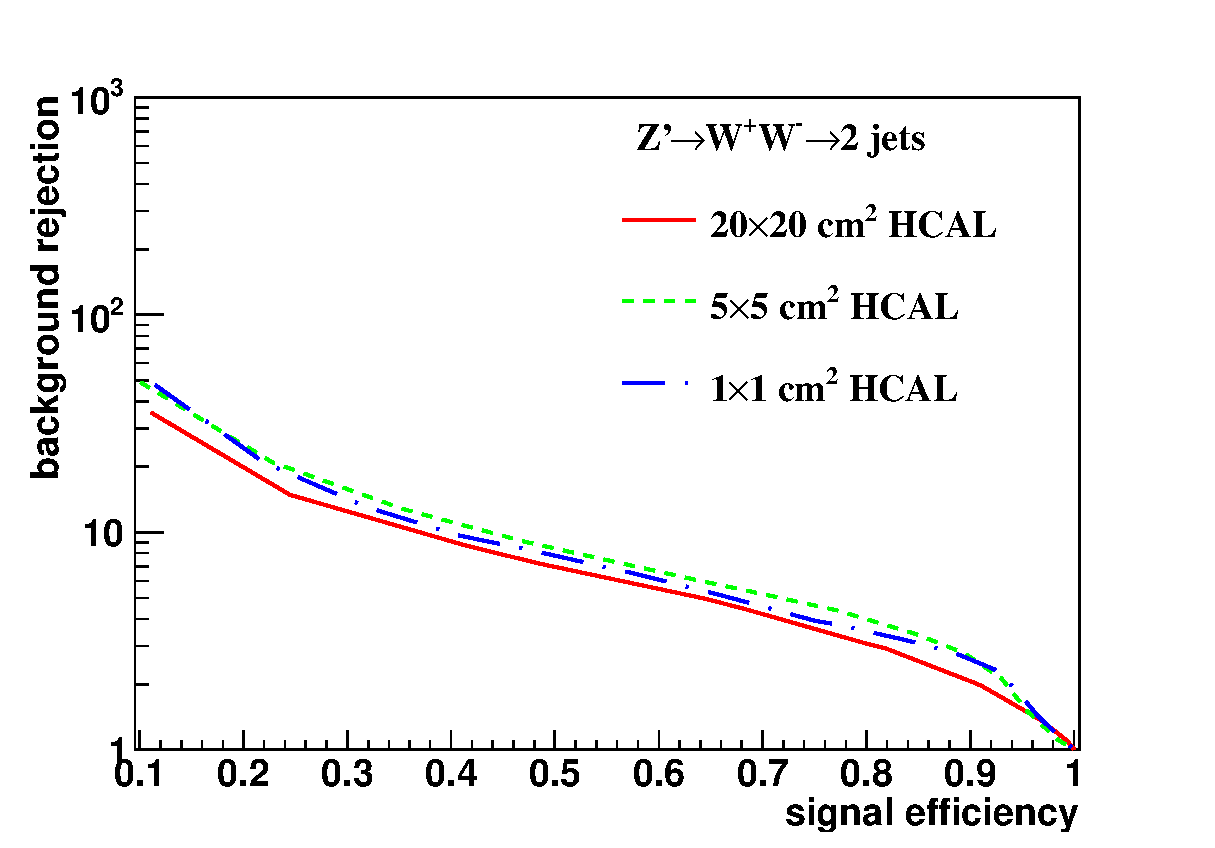
\includegraphics[width=0.43\textwidth]{ROC_Tau_C/Rawhit_05GeV_tau21_5tev_eff_1_New2_after_cut_25bins_no_mass_cut_new_75pa.eps}
   }
   \subfigure[Z'(10 TeV)] {
   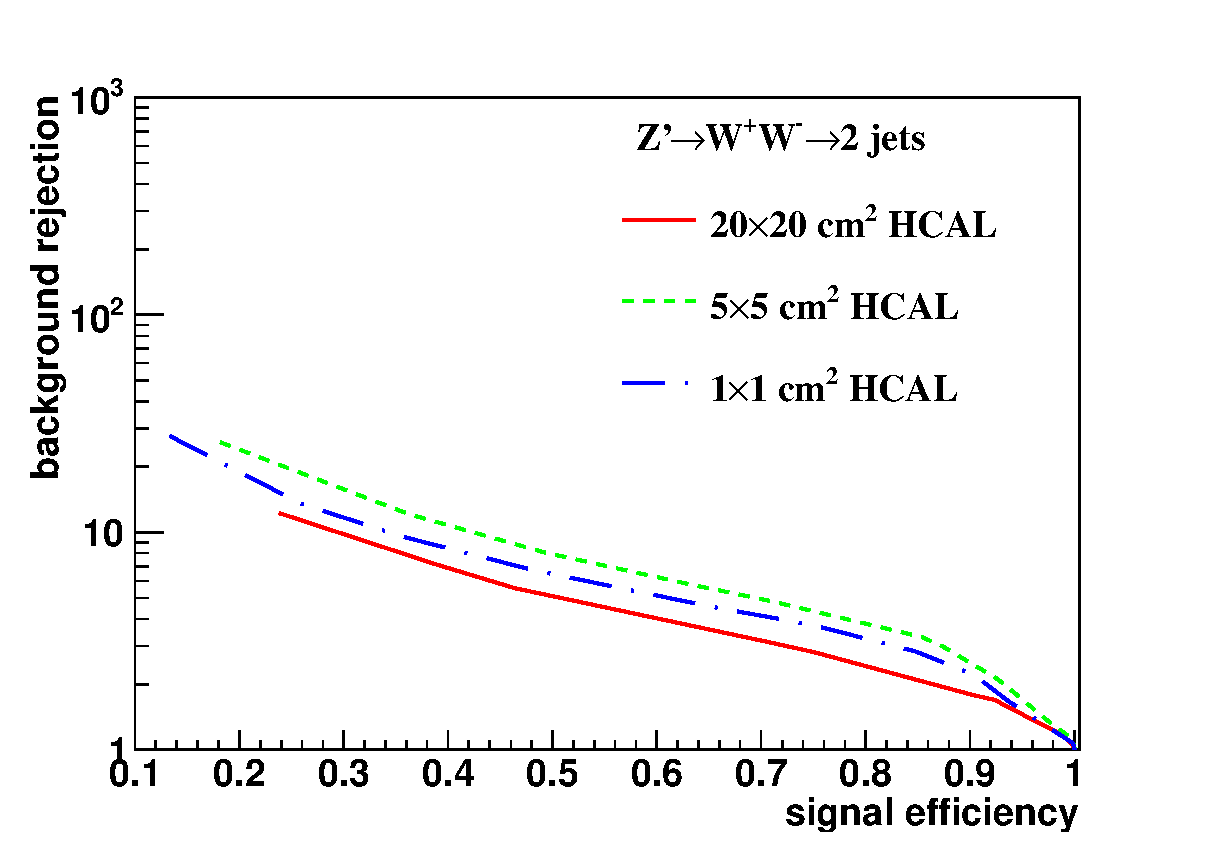
\includegraphics[width=0.43\textwidth]{ROC_Tau_C/Rawhit_05GeV_tau21_10tev_eff_1_New2_after_cut_25bins_no_mass_cut_new_75pa.eps}
   }
   \subfigure[Z'(20 TeV)] {
   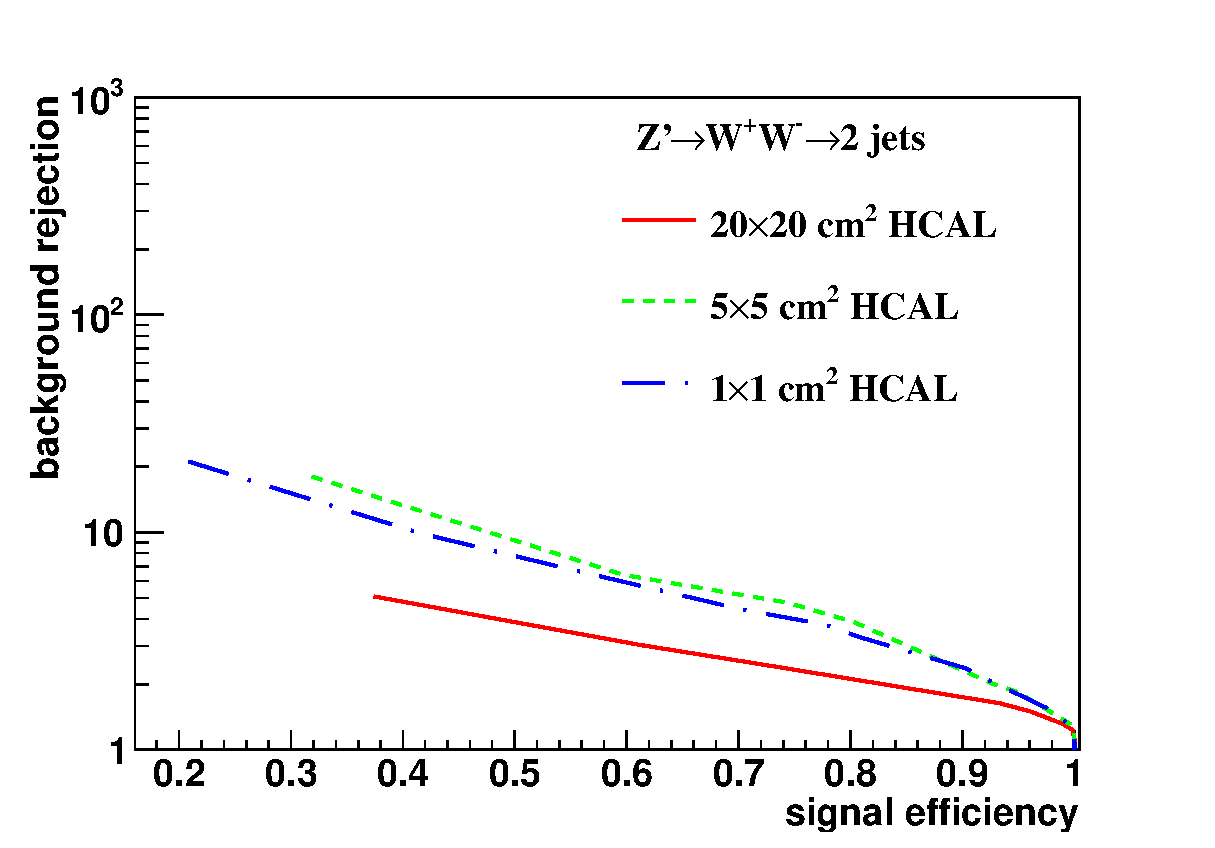
\includegraphics[width=0.43\textwidth]{ROC_Tau_C/Rawhit_05GeV_tau21_20tev_eff_1_New2_after_cut_25bins_no_mass_cut_new_75pa.eps}
   }
   \subfigure[Z'(40 TeV)] {
   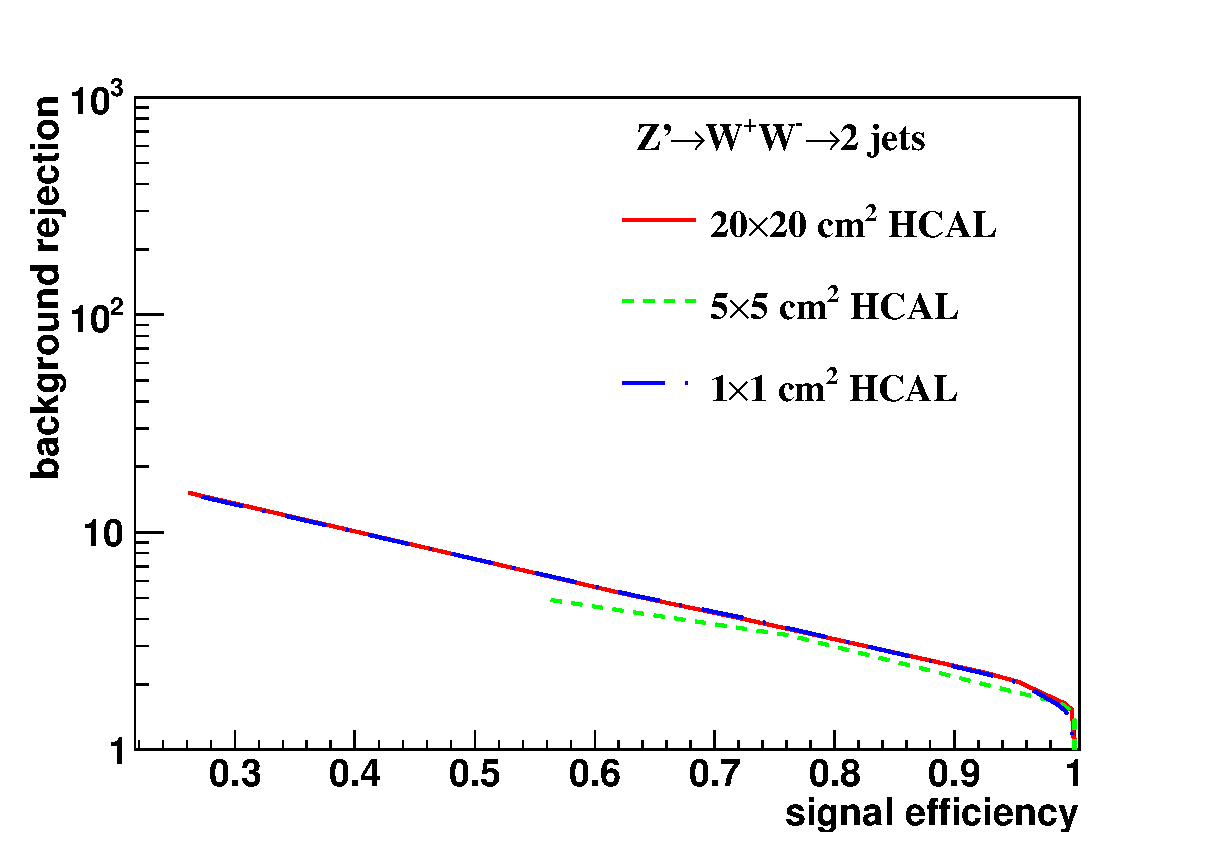
\includegraphics[width=0.43\textwidth]{ROC_Tau_C/Rawhit_05GeV_tau21_40tev_eff_1_New2_after_cut_25bins_no_mass_cut_new_75pa.eps}
   }
\end{center}
\caption{Signal efficiency versus background rejection rate using $\tau_{21}$.
The energies of collision at (a) 5, (b) 10, (c) 20, and (d) 40~TeV are shown 
here. 
In each figure, the three ROC curves correspond to different detector sizes.
\label{fig:Rawhit_05GeV_tau21_ROC}
}
\end{figure}


\begin{figure}
\begin{center}
   \subfigure[Z'(5 TeV)] {
   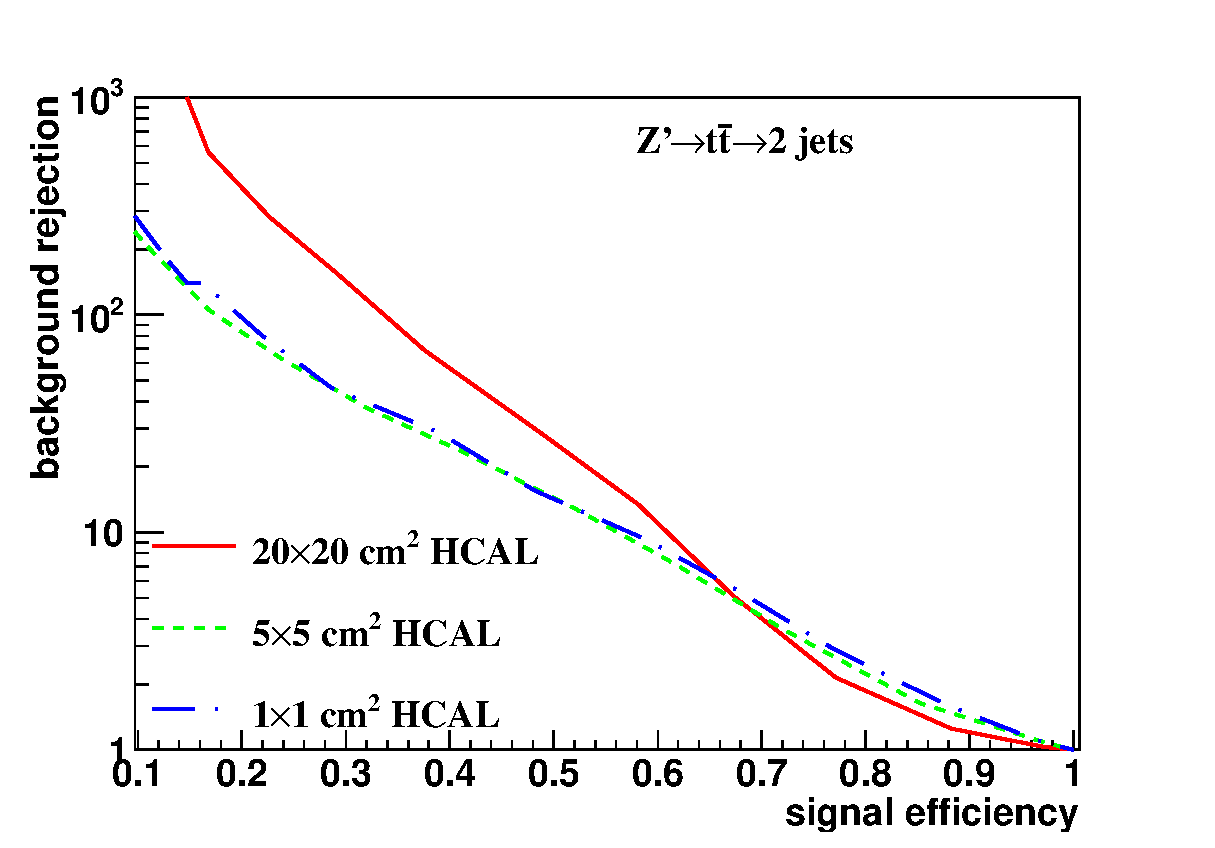
\includegraphics[width=0.43\textwidth]{ROC_Tau_C/Rawhit_05GeV_tau32_5tev_eff_1_New2_after_cut_25bins_no_mass_cut_new_75pa.eps}\hfill
   }
   \subfigure[Z'(10 TeV)] {
   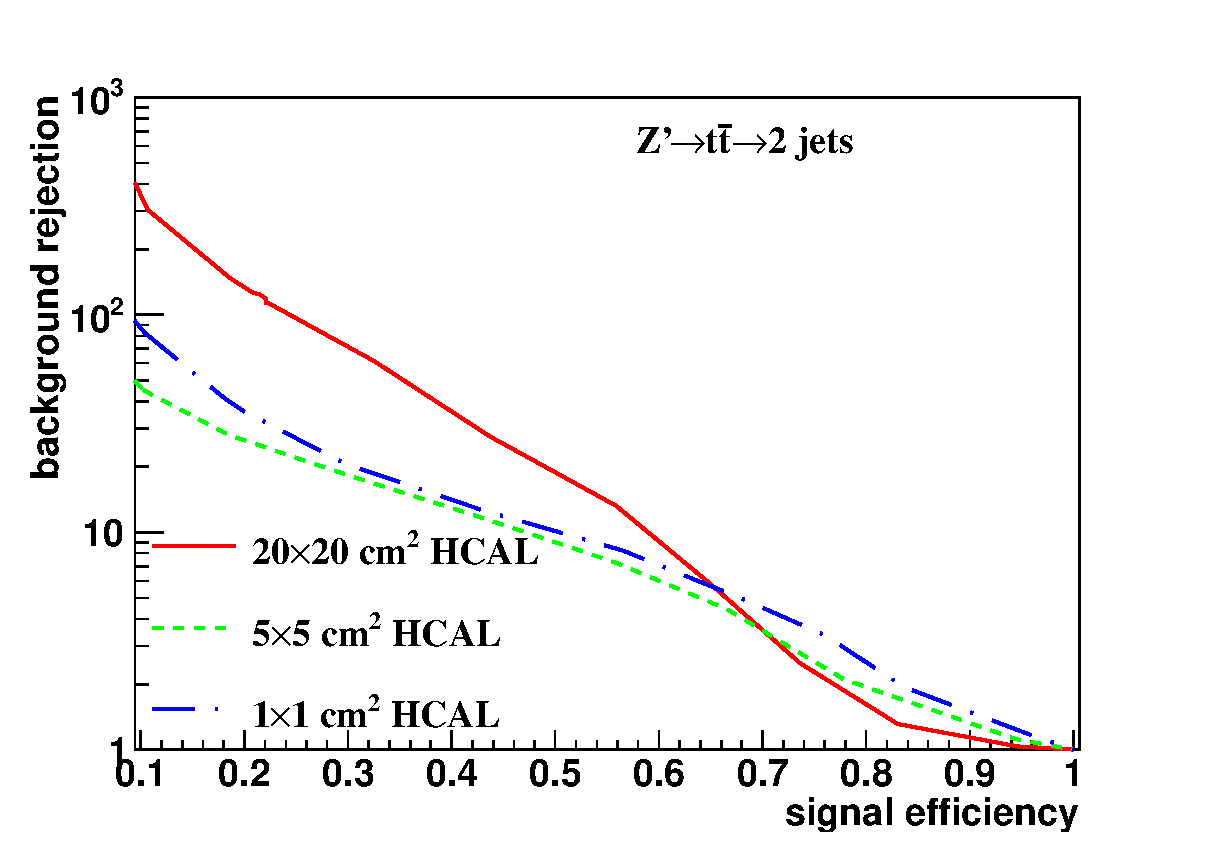
\includegraphics[width=0.43\textwidth]{ROC_Tau_C/Rawhit_05GeV_tau32_10tev_eff_1_New2_after_cut_25bins_no_mass_cut_new_75pa.eps}
   }
   \subfigure[Z'(20 TeV)] {
   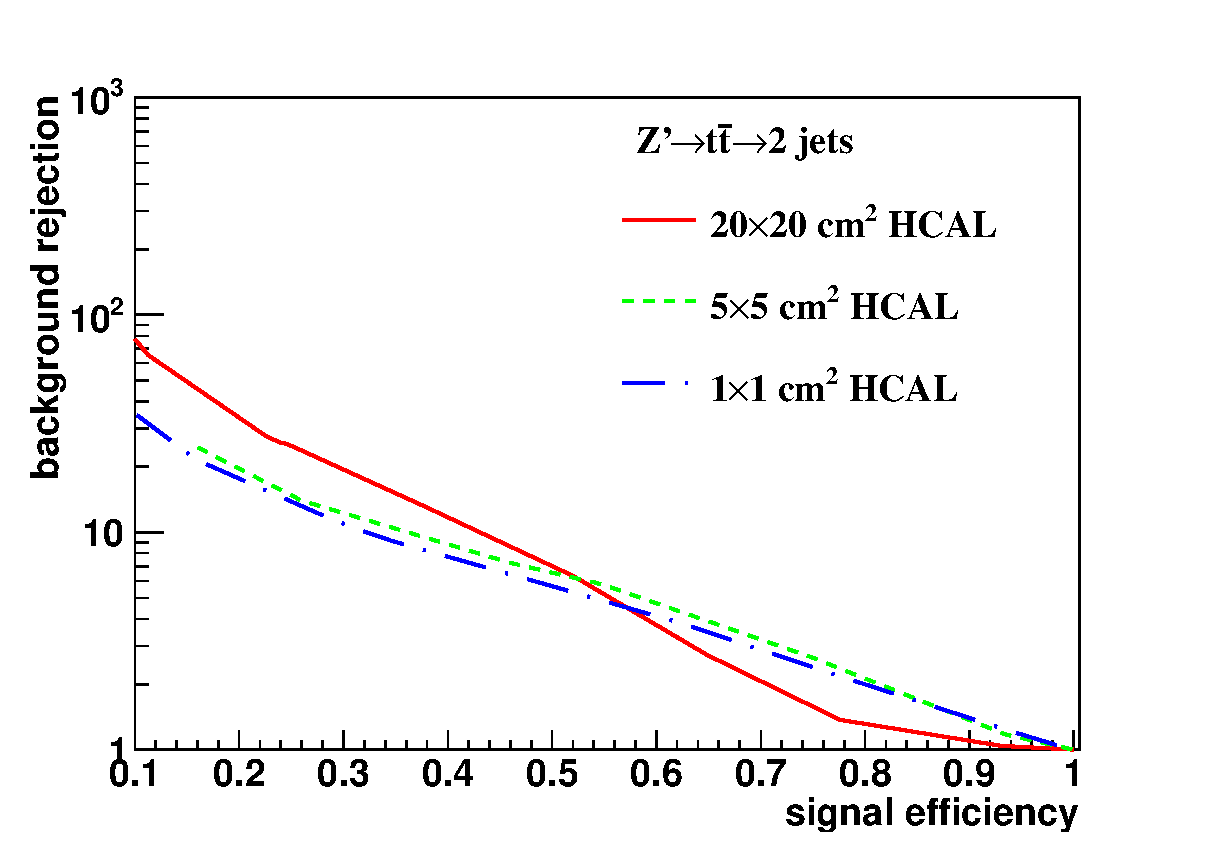
\includegraphics[width=0.43\textwidth]{ROC_Tau_C/Rawhit_05GeV_tau32_20tev_eff_1_New2_after_cut_25bins_no_mass_cut_new_75pa.eps}
   }
   \subfigure[Z'(40 TeV)] {
   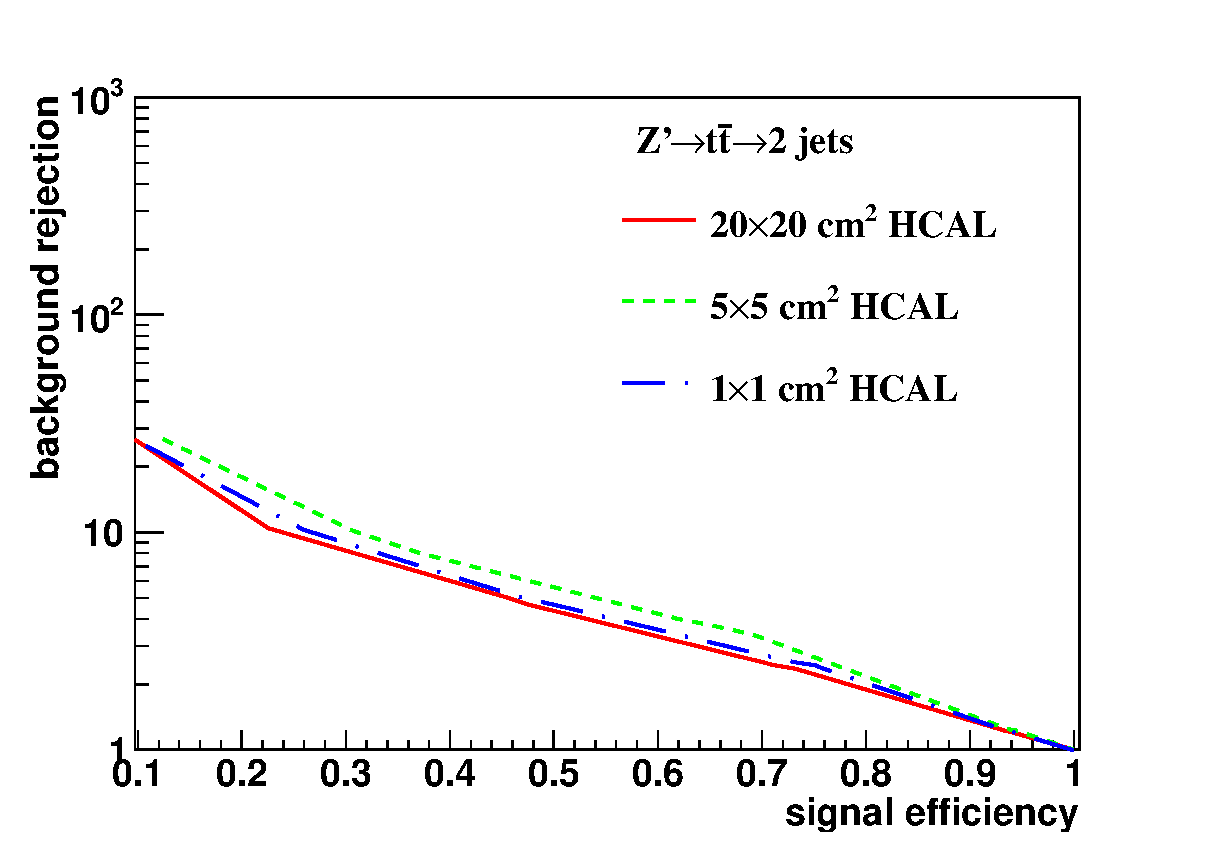
\includegraphics[width=0.43\textwidth]{ROC_Tau_C/Rawhit_05GeV_tau32_40tev_eff_1_New2_after_cut_25bins_no_mass_cut_new_75pa.eps}
   }
\end{center}
\caption{Signal efficiency versus background rejection rate using $\tau_{32}$. 
The energies of collision at (a) 5, (b) 10, (c) 20, and (d) 40~TeV are shown 
here. In each figure, the three ROC curves correspond to different detector 
sizes.
\label{fig:Rawhit_05GeV_tau32_ROC}
}
\end{figure}

\begin{figure}
\begin{center}
   \subfigure[Z'(5 TeV)] {
   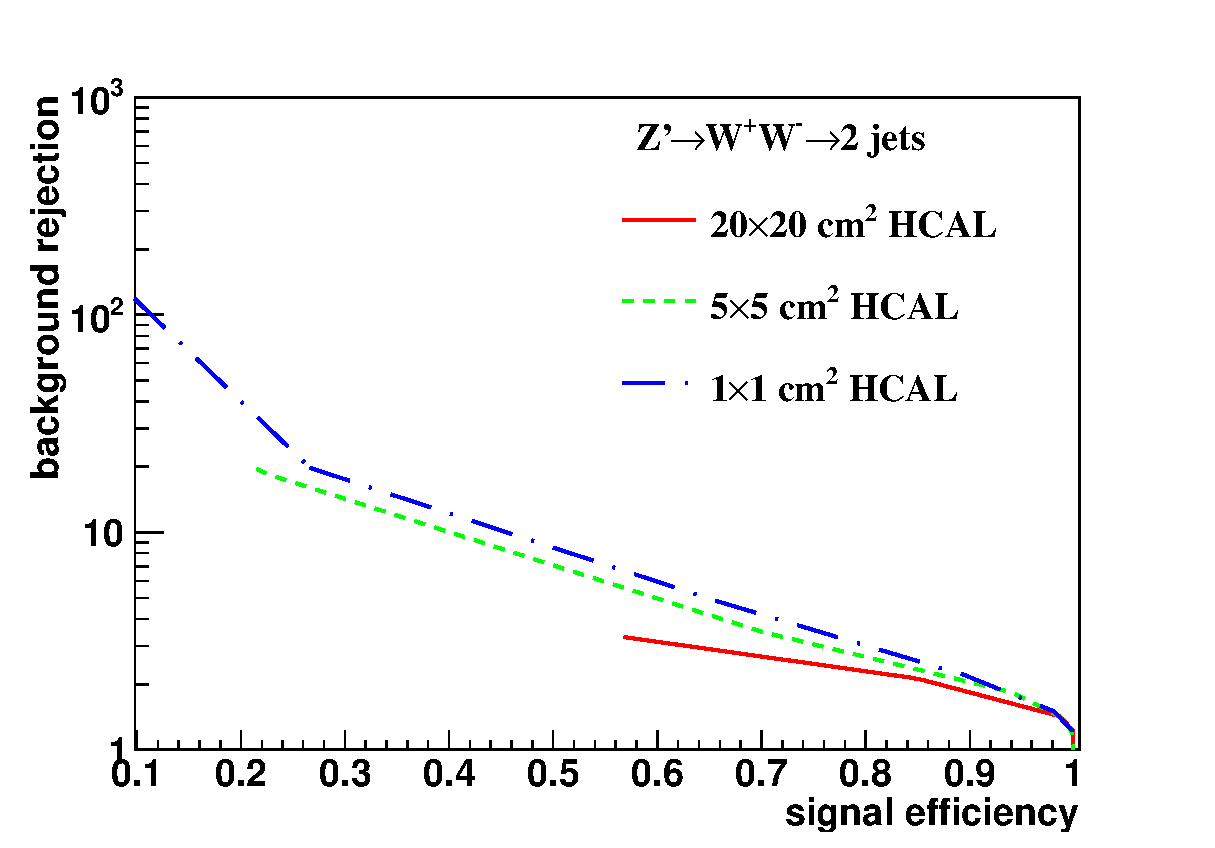
\includegraphics[width=0.43\textwidth]{ROC_Tau_C/Rawhit_05GeV_c2b1_5tev_eff_1_New2_after_cut_25bins_no_mass_cut_new_75pa.eps}\hfill
   }
   \subfigure[Z'(10 TeV)] {
   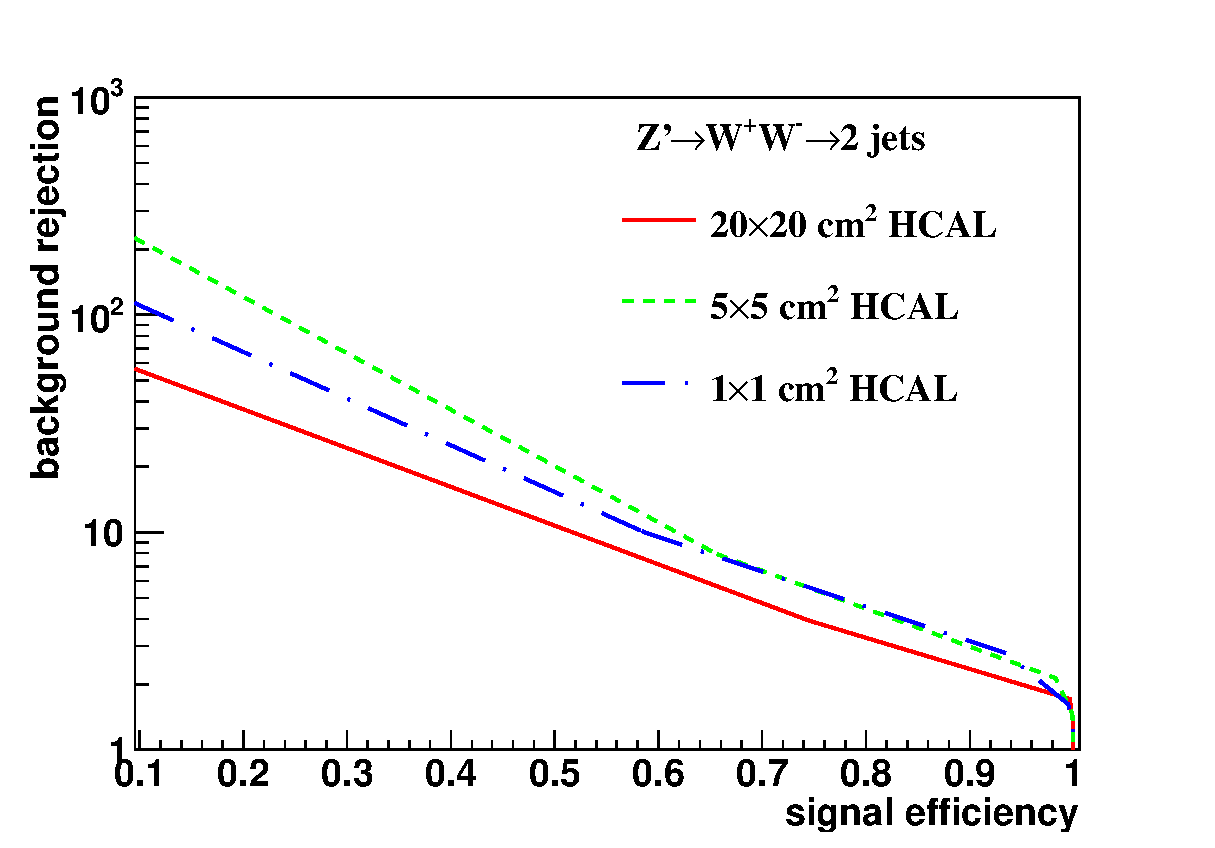
\includegraphics[width=0.43\textwidth]{ROC_Tau_C/Rawhit_05GeV_c2b1_10tev_eff_1_New2_after_cut_25bins_no_mass_cut_new_75pa.eps}
   }
   \subfigure[Z'(20 TeV)] {
   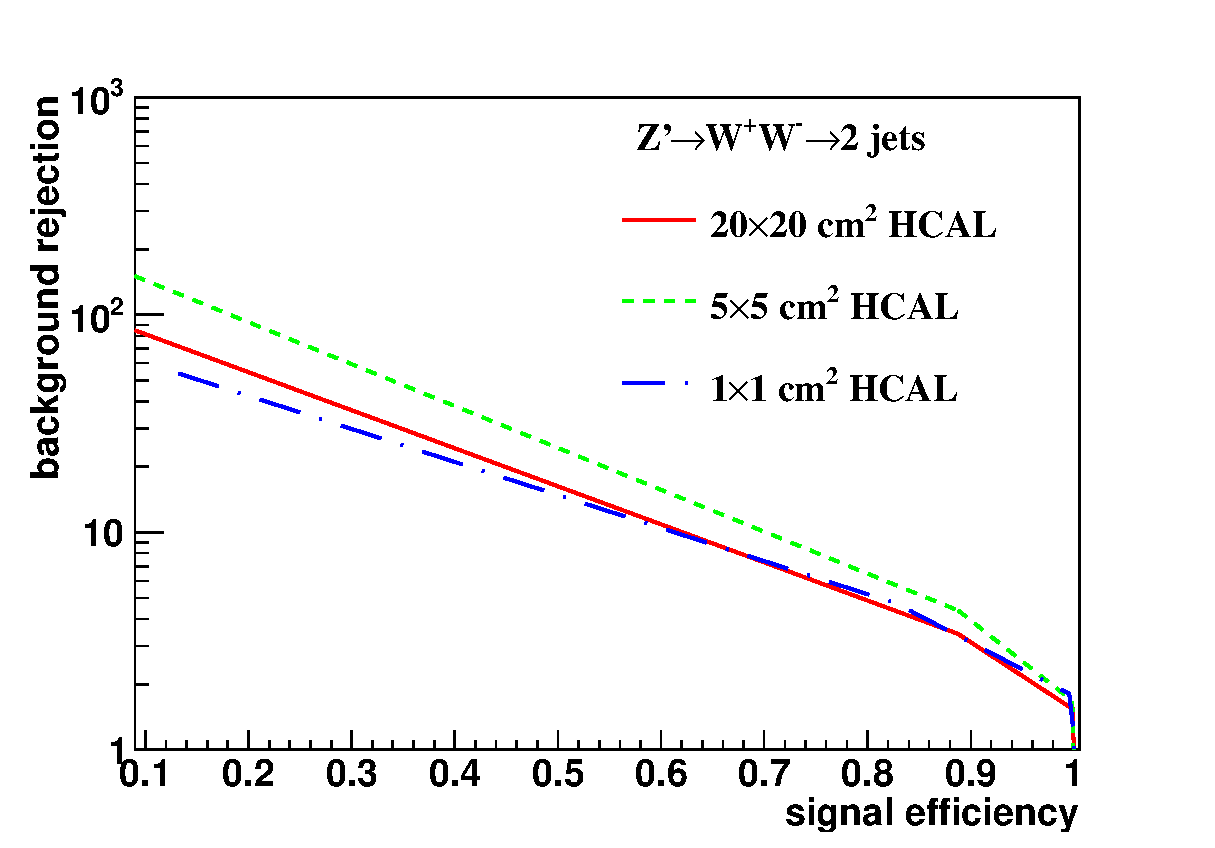
\includegraphics[width=0.43\textwidth]{ROC_Tau_C/Rawhit_05GeV_c2b1_20tev_eff_1_New2_after_cut_25bins_no_mass_cut_new_75pa.eps}
   }
   \subfigure[Z'(40 TeV)] {
   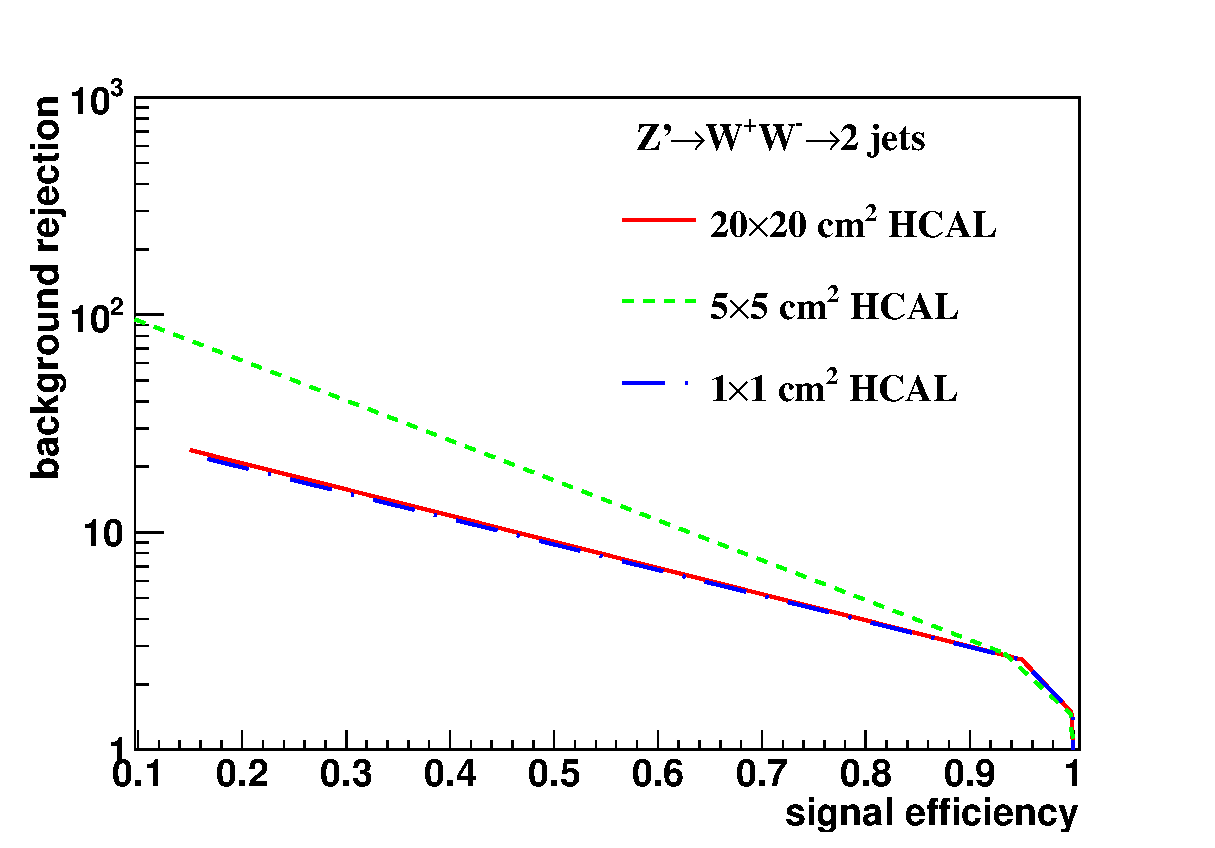
\includegraphics[width=0.43\textwidth]{ROC_Tau_C/Rawhit_05GeV_c2b1_40tev_eff_1_New2_after_cut_25bins_no_mass_cut_new_75pa.eps}
   }
\end{center}
\caption{Signal efficiency versus background rejection rate using $C_{2}^{1}$. 
The energies of collision at (a) 5, (b) 10, (c) 20, and (d) 40~TeV are shown 
here. In each figure, the three ROC curves correspond to different detector 
sizes.}
\label{fig:Rawhit_05GeV_c2b1_ROC}
\end{figure}

\end{document}






